\section{Raccolta dati}

I dati riguardanti la simulazione sono stati raccolti a partire dall'1 marzo 2020 fino al 27 giugno 2020 per un arco di tempo di circa 4 mesi, al ritmo di 1 richiesta al minuto dalle 7:00 alle 23:59 di ogni giorno.

\subsection{Le problematiche}

Sebbene questo studio fosse stato pensato per un confronto in condizioni di traffico e congestione stradale abituali che caratterizzano Milano, a influenzare questo studio è stato da subito l'emergenza epidemiologica da COVID-19. Il 22 gennaio 2020 il Governo Italiano ha dichiarato lo stato di emergenza, mettendo in atto le prime misure di contenimento in alcuni Comuni dove si sono verificati i primi casi del contagio. A partire dal 23 febbraio sono stati emanati DPCM (decreto del Presidente del Consiglio dei ministri) sempre più stringenti riguardo la circolazione e lo svolgimento delle attività commerciali, fino a ordinare un lockdown nazionale l'11 marzo 2020 \cite{misuredelgovernopercovid}. Nonostante lo studio sia stato fortemente influenzato da questo fattore, per via della circolazione ridotta se non totalmente assente durante il lockdown e per la riduzione del numero dei mezzi pubblici ATM, si è deciso comunque di procedere, tenendo conto dell'avvenuto sul giudizio finale dei risultati. A ostacolare lo studio, inoltre, nei primi giorni di utilizzo del programma per eseguire le richieste, è stato il servizio precedentemente utilizzato per i mezzi pubblici, ovvero Moovit, che ha risposto alle richieste con valori nulli o totalmente fuori scala. Per questo motivo è stato sostituito il servizio con quello offerto da Here e sono stati scartati i risultati precedentemente raccolti.

\subsection{Filtro dati errati}

I dati raccolti dalla prima esecuzione del programma, avvenuta l'1 marzo 2020, fino all'entrata in vigore dello stato di lockdown nazionale, il 12 marzo 2020, sono risultati per la maggior parte errati, ovvero con stime di percorrenza nulle, causati dai problemi con lo scraper di Moovit. Successivamente a questo evento si è cercato e trovato un servizio alternativo che sostituisse la stima del percorso coi mezzi pubblici, ovvero Here, che sfortunatamente non offre stime in tempo reale ma solo statiche. I dati raccolti nel periodo di lockdown dal 13 marzo 2020 al 3 maggio 2020 compresi sono stati scartati per via della circolazione dei mezzi pubblici e privati quasi totalmente assente, e quindi poco utili nell'obbiettivo finale dello studio di confrontare i mezzi di trasporto in situazioni di traffico caratteristico della città. Per questo motivo si è scelto di usare solamente i dati a partire dall'allentamento delle misure di restrizioni da emergenza sanitaria, ovvero quelli a partire dal 4 maggio 2020. Anche i dati presi in considerazione da quest'ultima data contengono delle stime nulle. Questo fenomeno è stato probabilmente dovuto alla generazione a random delle coordinate di partenza e arrivo, che ha permesso richieste in qualsiasi punto della mappa, compresi punti non situati direttamente sulla strada come in giardini pubblici, condomini e altre zone private, o semplicemente dovuto a disservizi. Per un confronto alla pari sono state considerate solo le righe prive di zeri nel file formato CSV. Come indicato dalla Tabella \ref{table:1} su circa 68000 richieste, 50000 sono prive di errori, circa il 73\% del totale, e quindi adatte per un confronto 1 a 1 tra mezzi di trasporto.

\begin{table}
	\centering
	\begin{tabular}{ | l | r | r | }
		\hline
		& \textbf{1 Marzo - 12 Marzo} & \textbf{4 Maggio - 27 Giugno} \\
		\hline
		\textbf{Coerenti}& 1988 & 49560 \\  
		\textbf{Errati} & 7962 & 18290 \\
		\hline
		\textbf{Totale} & 9680 & 67850 \\
		\textbf{\% Errati} & 79.5 & 27.0 \\
		\hline
	\end{tabular}
	\caption{Dati errati che contengono uno o più valori nulli nelle stime}
	\label{table:1}
\end{table}

\subsection{Salvataggio}

Nella Tabella \ref{table:7} è riportato l'header del file CSV in cui sono stati salvati i dati. Nei campi di partenza e arrivo sono state salvate le coordinate espresse in gradi del tragitto generato, nei restanti campi le stime di percorrenza di tale tragitto espresse in minuti, insieme alla data e all'orario in cui è stata effettuata la richiesta di tale tratta. Oltre ai dati principali sono state salvate informazioni secondarie come il numero di auto libere Enjoy al momento della richiesta, la lunghezza in via aerea della tratta e quella totale del percorso di ogni mezzo, tutte espresse in chilometri.

\begin{table}[H]
	\centering
	\begin{tabular}{ | c | c | c | c | c | c | c | c | c | }
		\hline
		Data & Orario & Partenza & Arrivo & Auto & ATM & Enjoy & Bici & Piedi \\
		\hline
	\end{tabular}
	\caption{Header del file CSV con i dati salvati}
	\label{table:7}
\end{table}

\subsection{Distribuzione lunghezza tratte generate}

Nella Figura \ref{image:2} e nella Tabella \ref{table:2} sono riportate le statistiche riguardo la lunghezza in via aerea delle tratte generate. Si può notare come più della metà siano lunghe meno di 5 km in linea aerea, risultato voluto e ottenuto dai vincoli imposti nella generazione riguardanti l'area del Comune di Milano e per l'ingresso e l'uscita dal centro storico al semicentro. La Figura \ref{image:19} mostra come la lunghezza delle tratte è stata equidistribuita nelle diverse fasce di orario.

\begin{figure}[H]
	\centering
	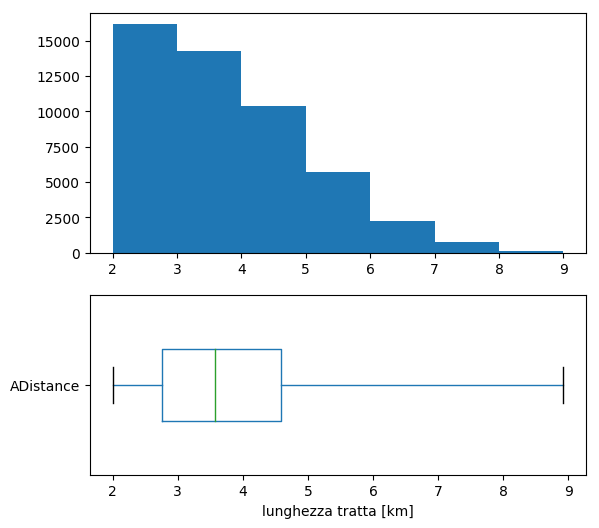
\includegraphics[scale=0.8]{distribuzione_tratte}
	\caption{Frequenza assoluta e distribuzione lunghezza tratte [km]}
	\label{image:2}
\end{figure}

\begin{figure}[H]
	\centering
	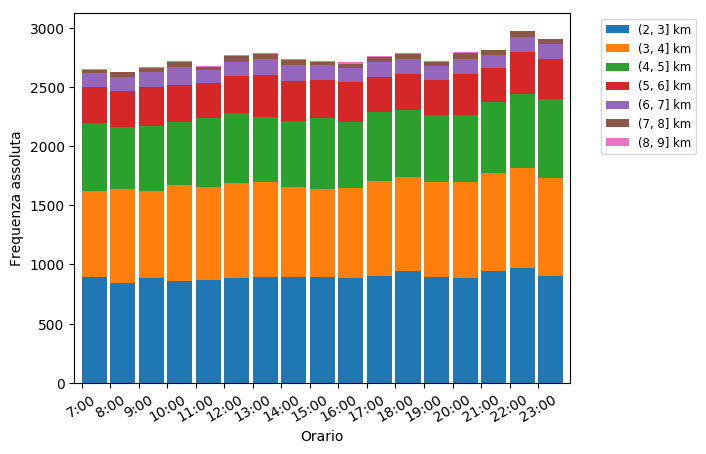
\includegraphics[scale=0.8]{distribuzione_tratte_oraria}
	\caption{Frequenza assoluta lunghezza tratte in base all'orario [km]}
	\label{image:19}
\end{figure}

\begin{table}[H]
	\centering
	\begin{tabular}{ | l r | }
		\hline
		\textbf{Abs. freq.} & 49560 \\
		\textbf{Media} & 3.80 km \\
		\textbf{Mediana} & 3.57 km \\
		\textbf{Std} & 1.27 km \\
		\textbf{Min} & 2.00 km \\
		\textbf{Max} & 9.52 km \\
		\hline
	\end{tabular}
	\caption{Statistiche lunghezza tratta [km]}
	\label{table:2}
\end{table}

\section{Performance dei singoli mezzi}

Dalla Figura  \ref{image:26} si può subito notare come i tragitti a piedi e in bicicletta abbiano dei baffi molto corti se non totalmente assenti rispetto agli altri mezzi, con conseguente varianza molto bassa, il che è un risultato aspettato dato che non c'è nessun fattore oltre la distanza a influenzare drasticamente il tempo di percorrenza per questi metodi di spostamento, motivo per cui i provider si limitano a calcolarne una stima statica.

\begin{table}
	\centering
	\begin{tabular}{ | l r r r r r | }
		\hline
		& \textbf{Auto} & \textbf{Enjoy} & \textbf{Bici} & \textbf{ATM} & \textbf{Piedi} \\
		\textbf{Media}      & 23.7 & 16.4 & 11.9 & 10.3 & 4.5 \\
		\textbf{Mediana} & 23.6 & 16.2 & 11.9 &   9.8 & 4.5 \\
		\textbf{Std}             &  3.9 &   4.2 &   1.3 &    3.0 & 0.0 \\
		\textbf{Min}            &  8.9 &   3.5 &   6.5 &    3.7 & 4.3 \\
		\textbf{Max}         & 59.0 & 46.4 & 16.9 &  41.0 & 4.6 \\
		\hline
	\end{tabular}
	\caption{Statistiche velocità media [km/h]}
	\label{table:3}
\end{table}

 Risultato opposto invece è stato ottenuto per i tragitti in auto, car sharing e mezzi pubblici, che mostrano una varianza molto più alta, come riportato nella Tabella \ref{table:3}, dovuta alla presenza di diverse variabili nel calcolo del tragitto. Nonostante le stime di percorrenza dei mezzi pubblici siano state calcolate dal provider usando solamente le tabelle degli orari dei mezzi, la varianza è risultata comunque alta per via delle numerosi variabili che influiscono sul tempo di percorrenza, come la distanza tra il punto di partenza e la fermata del mezzo, la scelta stessa del tipo di mezzo, come bus, tram o metro, e la corrispettiva velocità nominale. Questi primi risultati sono in linea con quelli dell'ISFORT riportati nella Tabella \ref{table:9}, che vede l'automobile in testa alla classifica intorno a 22 km/h di media, con la bici al secondo posto ma con 15 km/h e i mezzi pubblici al terzo con 14 km/h, stime poco più alte di quelle sopra riportate.

\begin{figure}
\centering
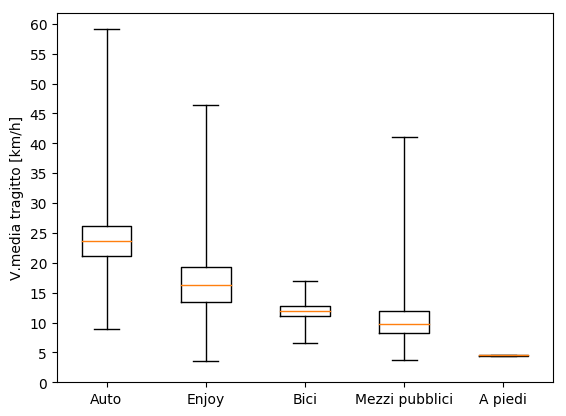
\includegraphics[scale=0.7]{vmedia_all}
\caption{Distribuzione velocità media dei singoli mezzi}
\label{image:26}
\end{figure}

\pagebreak

\subsection{Automobile}

\subsubsection{Velocità media}

Una delle prime analisi effettuate per ogni mezzo è stata quella di calcolare la velocità media per ogni tragitto effettuato riguardante l'intero periodo di raccolta dati, con l'obbiettivo di osservare eventuali variazioni di ora in ora. Come riportato nella Figura \ref{image:3}, si evidenziano due situazioni, caratterizzate da una differenza nella velocità media: più bassa nelle fasce di orario delle 8:00-11:00 e delle 17:00-19:00, in cui è stata registra la velocità media minima di 23 km/h, e più alta nelle ore restanti. La massima velocità media invece è stata rileva nei tragitti dopo le 22:00, di circa 26 km/h. Tali risultati sono in linea, tra i tanti studi a riguardo del traffico in auto a Milano, con quelli dello studio di TomTom\footnote{\url{https://www.tomtom.com/en_gb/traffic-index/ranking/}. Accessed: 20/01/2021} effettuato sulla città di Milano nel 2019, che evidenzia le 9:00 e le 18:00 come orari di picco del traffico stradale dal lunedì al venerdì, con un livello di congestione rispettivamente del 70\% e del 60\%.

\begin{figure}[H]
	\centering
	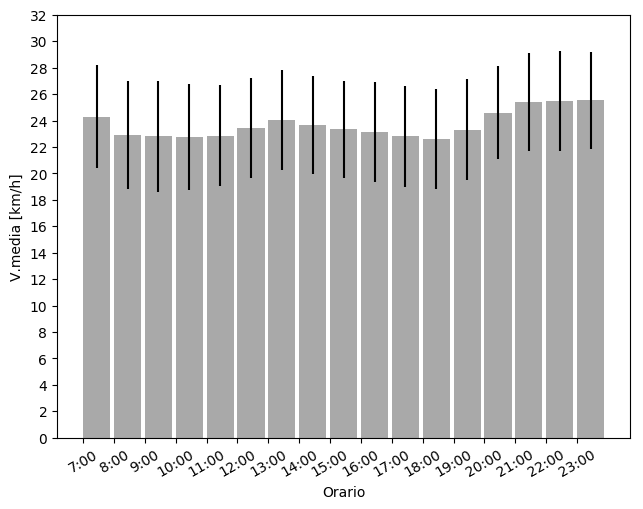
\includegraphics[scale=0.8]{vmedia_oraria_auto}
	\caption{Velocità media in auto [km/h] di ora in ora. I baffi neri rappresentano la deviazione standard campionaria $\sigma$ rispettiva di ogni barra}
	\label{image:3}
\end{figure}

Risultano in linea con lo studio anche le ore precedenti e successive agli orari individuati come picchi. Si nota inoltre come le deviazioni standard campionarie di ogni ora, rappresentate da baffi neri incastonati nelle barre, rimangano invariate. Si è scelto di rappresentare la deviazione standard invece che l'errore standard per via dell'elevata numerosità del campione che renderebbe i baffi non visibili e quindi non distinguibili. Difatti, basandosi sui dati della Tabella \ref{table:3} che riporta una deviazione standard di 3.9 e nella Figura \ref{image:19} che mostra una media di circa 2600 tratte per ogni fascia di orario, l'errore standard per ogni barra risulterebbe di: $\frac{\sigma_x}{\sqrt{n}} = \frac{3.9}{\sqrt{2600}} = 0.07$.



\subsubsection{Velocità media lunedì-venerdì e sabato-domenica}

La Figura \ref{image:4} mostra il risultato di una ripartizione dei dati effettuata sulla base del giorno della settimana, in particolare sono stati divisi i tragitti effettuati dal lunedì al venerdì da quelli del sabato e domenica. Per rendere leggibile la differenza è stata spostata l'origine del grafico al valore 16 sull'asse delle ordinate. 

\begin{figure}[H]
	\centering
	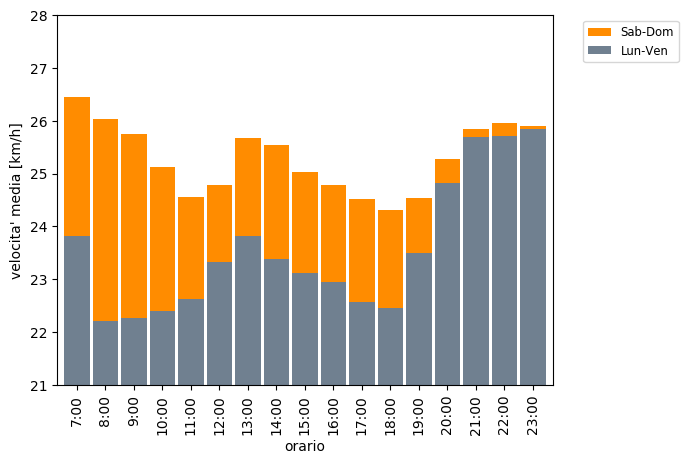
\includegraphics[scale=0.8]{vmedia_oraria_auto_weekend}
	\caption{Velocità media in auto [km/h] di ora in ora. I valori sull'asse delle ordinate variano tra 16 e 28}
	\label{image:4}
\end{figure}

La differenza è nel complesso bassa, di circa 2 km/h di media, che tende a diminuire nel primo pomeriggio e negli orari notturni e ad aumentare nella fascia oraria delle ore 8;00 e delle 16:00, con una differenza di quasi 4 km/h, equivalente a un incremento della velocità media nel fine settimana del 14.6\% in più rispetto al lunedì-venerdì. La variazione della velocità media di ora in ora nel sabato-domenica risulta meno evidente di quella del lunedì-venerdì, con i picchi di rallentamento che si spostato nelle fasce orarie 10:00-12:00 e 16:00-19:00. Anche questi dati risultano in linea con quelli dello studio di TomTom, che vede un minor livello di congestione nel weekend con dei picchi nelle ore 10:00 e 18:00. La deviazione standard delle fasce di orario del lunedì-venerdì e sabato-domenica, che sono state omesse per motivi di leggibilità del grafico, rimangono sempre costanti intorno al valore 3.7 km/h, con un errore standard di $\frac{3.7}{\sqrt{1622}} = 0.09$ per i giorni dal lunedì al venerdì e $\frac{3.7}{\sqrt{622}} = 0.14$ per i fine settimana, dove 1622 e 622 rappresentano rispettivamente la numerosità del campione di una sola fascia di orario lunedì-venerdì e di sabato-domenica.

\subsubsection{Velocità media settimana dopo settimana da fine lockdown}

La Figura \ref{image:5} mostra il risultato di una ripartizione dei dati effettuata in base alla settimana, in particolare sono stati partizionati a gruppi di 2 settimane consecutive i tragitti effettuati a partire dal 4 maggio 2020, primo giorno dell'allentamento delle restrizioni imposte dal governo italiano per l'emergenza COVID-19 \cite{misuredelgovernopercovid}. Nel grafico risulta evidente una degradazione della velocità media generale e lineare rispetto al passare delle settimane. Si nota inoltre che le curve corrispondenti alle settimane successive al 17 maggio, ovvero dopo le prime 2, presentino dei flessi sempre più accentuati in prossimità degli orari di picco del traffico evidenziati dalla Figura \ref{image:3}. Anche in questo caso, non sono state riportate differenze nella deviazione standard. Nella Figura \ref{image:27} sono stati usati i box plot per descrivere la distribuzione delle velocità medie a gruppi di 2 settimane dalla fine del lockdown. Si può notare come il quartile zero, primo, secondo e terzo siano rimasti uguali, con un lieve andamento a ribasso col passare delle settimane. La differenza risulta più accentuata nel quarto quartile, che vede la diminuzione dei valori di massima velocità media per tragitto, probabilmente dovuta a un aumento del traffico, come emerso dal grafico della Figura \ref{image:5} con valori decrescenti della velocità media per ogni fascia di orario al passare delle settimane dalla fine del lockdown.

\begin{figure}
	\centering
	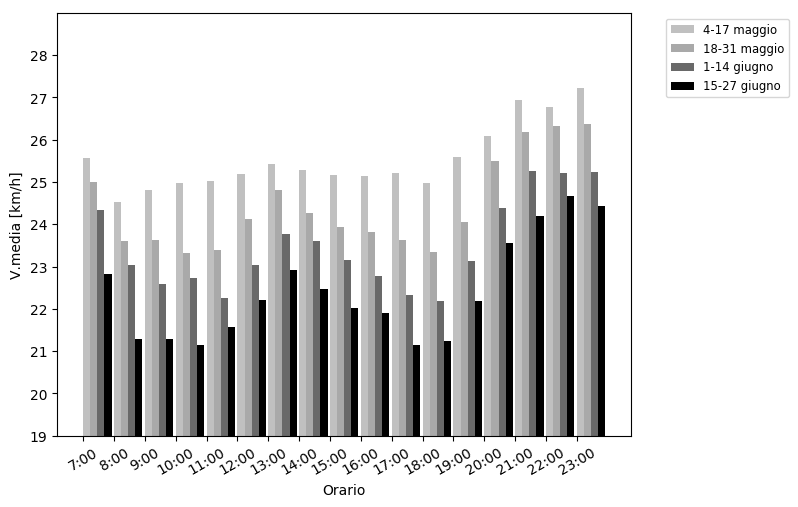
\includegraphics[scale=0.8]{vmedia_oraria_auto_weeks}
	\caption{Velocità media in auto [km/h] di ora in ora. I valori sull'asse delle ordinate variano tra 16 e 30}
	\label{image:5}
\end{figure}

\begin{figure}
	\centering
	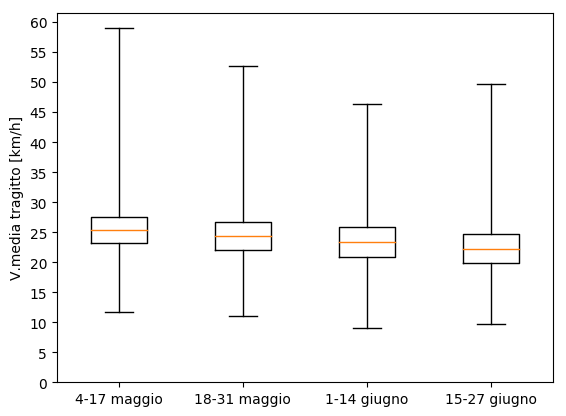
\includegraphics[scale=0.9]{vmedia_auto_weeks}
	\caption{Distribuzione della velocità media in auto [km/h] calcolata a gruppi di 2 settimane dalla fine del lockdown}
	\label{image:27}
\end{figure}

\subsubsection{Velocità media in base alla lunghezza del tragitto}

Nella Figura \ref{image:6} sono riportati, tramite una heatmap, i dati della velocità media divisi per fasce d'orario e per lunghezza della tratta. Si evidenziano due gobbe in corrispondenza degli orari di picco del traffico intorno alle ore 9:00 e 18:00, e le tratte brevi, lunghe dai 2 ai 3 chilometri, risultano le più colpite. Si evidenzia inoltre un'area di forma rettangolare di colori chiari a partire dalle ore 20:00, dove la velocità media si stabilizza intorno ai 27 km/h per le tratte superiori ai 3 km.

\begin{figure}[H]
	\centering
	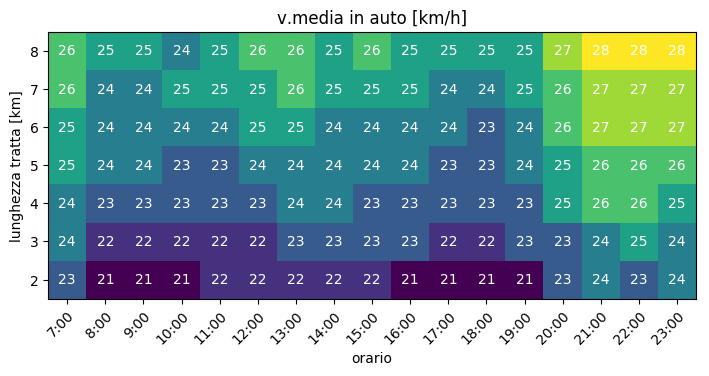
\includegraphics[scale=0.75]{heatmap_auto}
	\caption{Velocità media in auto [km/h] di ora in ora in base alla lunghezza della tratta}
	\label{image:6}
\end{figure}

\pagebreak

\subsection{Enjoy}

\subsubsection{Velocità media}

I tragitti col servizio di car sharing Enjoy hanno subito una lieve variazione di velocità media nell'arco 8:00-11:00 e in quello delle 17:00-19:00 in cui si è registrata la velocità media minima di 16 km/h e di 17 km/h di massima. La variazione è all'atto pratico poco significativa. La deviazione standard rimane costante per tutte le fasce di orario. Rispetto al grafico della Figura \ref{image:3} della velocità media in auto, la curva risulta molto simile, traslata verticalmente di 6 km/h. Anche in questo caso è stata usata la deviazione standard invece dell'errore standard per motivi di leggibilità, data l'elevata numerosità del campione.

\begin{figure}[H]
	\centering
	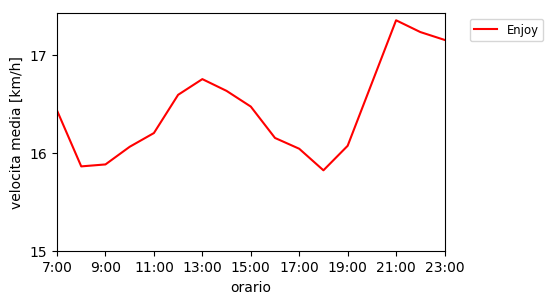
\includegraphics[scale=0.8]{vmedia_oraria_enjoy}
	\caption{Velocità media usando il car sharing Enjoy [km/h] di ora in ora.  I baffi neri rappresentano la deviazione standard campionaria $\sigma$ rispettiva di ogni barra}
	\label{image:7}
\end{figure}

\subsubsection{Velocità media lunedì-venerdì e sabato-domenica}

Non sono state registrate particolari differenze effettuando la ripartizione dei dati in base ai giorni dal lunedì al venerdì e del fine settimana, come mostrato nella Figura \ref{image:20}. La velocità media rimane costante, con una lieve differenza nella fascia oraria delle 8:00. La deviazione standard, rimane costante e identica a quella della Figura \ref{image:7} per tutte le fasce di orario.

\begin{figure}[H]
	\centering
	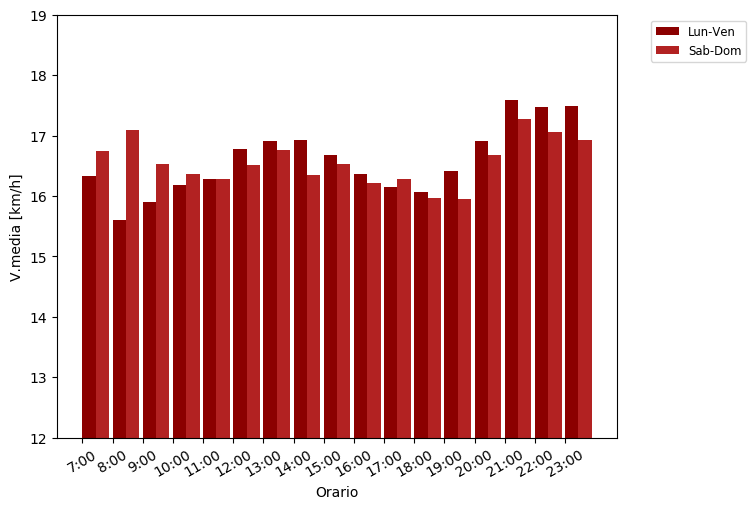
\includegraphics[scale=0.8]{vmedia_oraria_enjoy_weekend}
	\caption{Velocità media usando il car sharing Enjoy [km/h] di ora in ora. I valori sull'asse delle ordinate variano tra 12 e 21}
	\label{image:20}
\end{figure}

\subsubsection{Velocità media settimana dopo settimana da fine lockdown}

Anche per il car sharing risulta evidente una degradazione della velocità media generale e lineare rispetto al passare delle settimane, come riportato nel grafico della Figura \ref{image:16}. Non risultano differenze nelle fasce orarie meno trafficate dalle 12:00 alle 15:00 e dalle 21:00 alle 23:00. Le prime due settimane dall'allentamento delle restrizioni risultano più veloci di circa 1 km/h di media dalle altre settimane. Nel grafico della Figura \ref{image:28}, come per l'automobile di proprietà, il quartile zero, primo, secondo e terzo risultano uguali, con un andamento decrescente del baffo del quarto quartile entro cui ricadono i valori massimi di velocità media per tragitto, sempre dovuto con molta probabilità al traffico.

\begin{figure}[H]
	\centering
	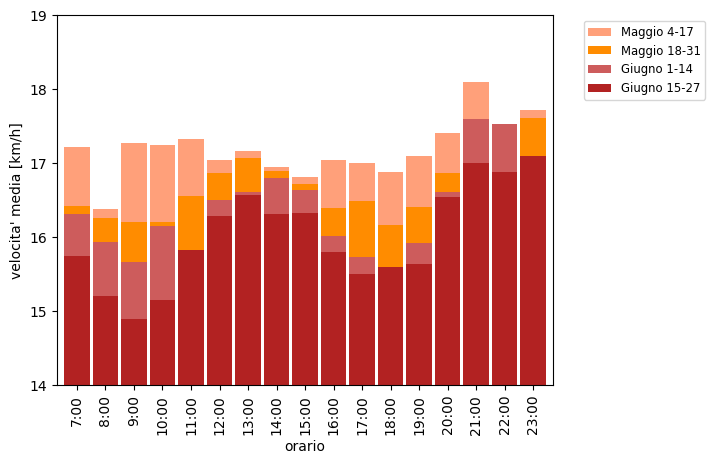
\includegraphics[scale=0.8]{vmedia_oraria_enjoy_weeks}
	\caption{Velocità media in car sharing Enjoy [km/h] di ora in ora. I valori sull'asse delle ordinate variano tra 12 e 21}
	\label{image:16}
\end{figure}

\begin{figure}
	\centering
	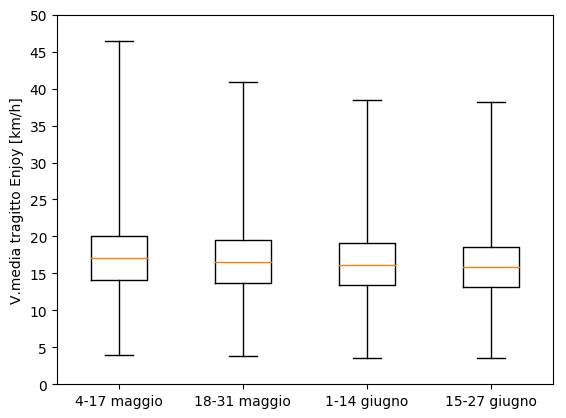
\includegraphics[scale=0.8]{vmedia_enjoy_weeks}
	\caption{Distribuzione della velocità media in car sharing Enjoy [km/h] calcolata a gruppi di 2 settimane dalla fine del lockdown}
	\label{image:28}
\end{figure}

\subsubsection{Velocità media in base alla lunghezza del tragitto}

Nel grafico della Figura \ref{image:30} sono riportati, tramite una heatmap, i dati della velocità media divisi per fasce d'orario e per lunghezza della tratta. In questo caso, a differenza della heatmap dell'auto di proprietà, corrispondente alla Figura \ref{image:6}, le velocità medie risultano mediamente costanti in base alla lunghezza della tratta, indipendentemente dall'orario, con lievi diminuzioni nelle ore intorno alle 9:00 e 18:00. A differenza dell'auto, la velocità media sembra non aumentare in corrispondenza degli orari notturni, questo probabilmente è dovuto al grande impatto che ha il tratto a piedi per raggiungere un mezzo libero della flotta.

\begin{figure}
	\centering
	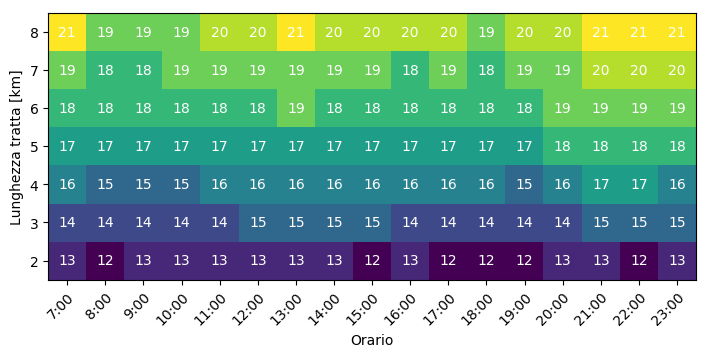
\includegraphics[scale=0.75]{heatmap_enjoy}
	\caption{Velocità media in car sharing Enjoy [km/h] di ora in ora in base alla lunghezza della tratta}
	\label{image:30}
\end{figure}

\subsubsection{Auto libere e tempo medio per raggiungerle}

Sottraendo il tempo impiegato in auto da quello impiegato col car sharing Enjoy è stata ottenuta una stima indicativa del tempo medio per raggiungere un'auto libera a piedi. Dai calcoli è risultato che il tempo medio oscilla intorno ai 6 minuti, come riportato dalla Tabella \ref{table:4}. Il box plot della Figura \ref{image:8} evidenzia il range interquartile nell'intervallo dai 3 ai 9 minuti, con una mediana di 6. Il tempo medio per raggiungere un'auto Enjoy, di 6.6 minuti, sembra coincidere con la differenza di velocità media rispetto ai dati dell'auto privata, citata a riguardo del grafico della Figura \ref{image:7}.

Anche per questa analisi i dati sono stati partizionati per i giorni da lunedì a venerdì e per sabato e domenica. Il grafico della Figura \ref{image:21} mostra una lieve differenza nel tempo medio per raggiungere un'auto libera Enjoy di circa 1 minuto a sfavore dei giorni del fine settimana. Dunque, in settimana, le auto sono risultate più facilmente raggiungibili.

Per contestualizzare il tempo medio per raggiungere un'auto Enjoy è stato usato il dato sul numero delle auto libere salvato per ogni richiesta ai servizi. Il massimo numero di auto libere in circolazione è stato di 870. Nella Figura \ref{image:9} viene mostrata in media la variazione di questo conteggio lungo l'arco della giornata, ripartito per lunedì-venerdì e sabato-domenica. Si può notare come il picco di utilizzo del servizio, denotato da un calo delle auto libere a disposizione, inizia verso le 15:00 e finisce verso le 21:00 indipendentemente dal giorno. L'unica differenza tra i due gruppi si può notare nelle ore del mattino, che vede meno auto libere durante la settimana. Il grafico della Figura \ref{image:10} mostra chiaramente come il numero delle auto libere a disposizione sia aumentato con la fine del lockdown. Si può notare infatti come siano state immesse circa 150 nuove auto nell'arco di un mese e altre 50 nel mese successivo. Questo dato è stato probabilmente dovuto al ritiro di una parte del parco auto da parte delle aziende per motivi di manutenzione, vista l'occasione della scarsa domanda di servizio.

\begin{table}[H]
	\centering
	\begin{tabular}{ | l r | }
		\hline
		& \textbf{T.medio ragg.auto} \\
		\textbf{Media}   &  6.6 \\
		\textbf{Mediana} &  6.0 \\
		\textbf{Std}     &  4.6 \\
		\textbf{Min}     &  0.0 \\ 
		\textbf{Max}     & 43.0 \\
		\hline
	\end{tabular}
	\caption{Statistiche tempo medio per raggiungere auto libera [min]}
	\label{table:4}
\end{table}

\begin{figure}[H]
	\centering
	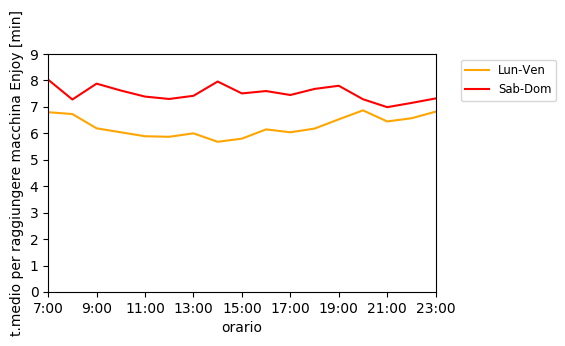
\includegraphics[scale=0.7]{tmedio_raggiungimento_auto_enjoy}
	\caption{Distribuzione del tempo impiegato a raggiungere auto libera [min]}
	\label{image:8}
\end{figure}

\begin{figure}
	\centering
	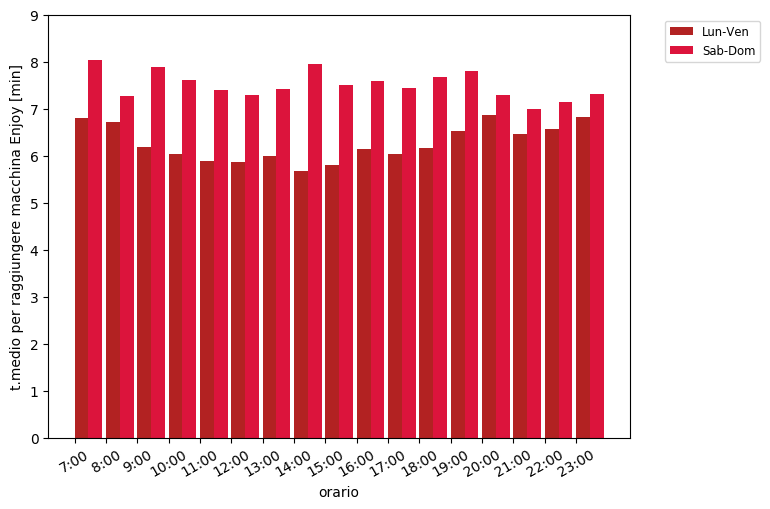
\includegraphics[scale=0.8]{tmedio_raggiungimento_auto_enjoy_weekend}
	\caption{Tempo medio per raggiungere auto libera [min]}
	\label{image:21}
\end{figure}

\begin{figure}
	\centering
	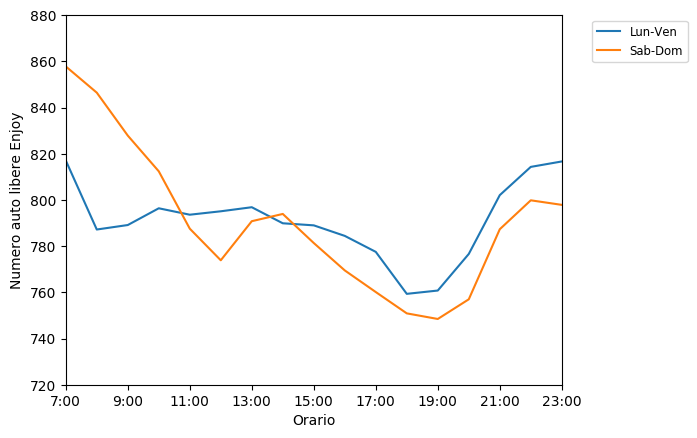
\includegraphics[scale=0.8]{variazione_auto_libere_enjoy_weekend}
	\caption{Numero di auto libere Enjoy lungo l'arco della giornata}
	\label{image:9}
\end{figure}

\begin{figure}
\centering
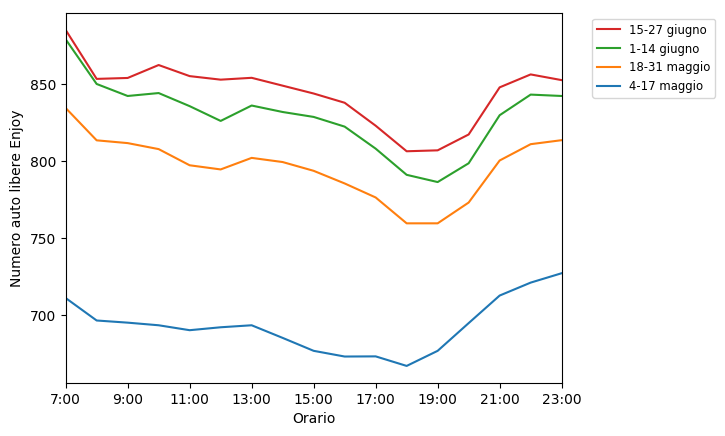
\includegraphics[scale=0.8]{variazione_auto_libere_enjoy_weeks}
\caption{Numero di auto libere Enjoy lungo settimana dopo settimana}
\label{image:10}
\end{figure}

\pagebreak

\subsection{Mezzi pubblici ATM, bici e a piedi}

Analizzando le stime di percorrenza riguardo i mezzi pubblici, la bicicletta e i percorsi a piedi, non si è verificata alcuna variazione significativa lungo l'arco della giornata, tradotto graficamente come nelle Figure \ref{image:11}, \ref{image:17} e \ref{image:18} in una retta parallela all'asse x per ognuno dei mezzi considerati. Il risultato è aspettato, dato che tali servizi non hanno fornito risposte dinamiche in base alle condizioni attuali del traffico e dei dati storici, e, nel caso della bicicletta e a piedi, perché l'influenza è praticamente nulla per questi mezzi di trasporto.

Si è deciso di analizzare ulteriormente le performance dei mezzi pubblici per via della loro grande varianza, al pari di quella dell'auto e del car sharing. Nel grafico della Figura \ref{image:29} è riportata un'analisi tramite box plot per visualizzare la distribuzione dei valori di velocità media di settimana in settimana dalla fine del lockdown. Dal risultato emerge un netto cambiamento del quarto quartile a partire dal 1 giugno 2020, che vede un accorciamento del baffo corrispondente ai valori massimi di velocità media registrati. Nel tentativo di trovare una risposta a questo cambiamento, dato che può dipendere solamente dal cambio delle tabelle degli orari dei mezzi, visto che le API Here usate per questo mezzo si basano solo su di esse, si è tentato di accedere agli archivi pubblici delle notizie riguardanti cambiamenti di servizio dal sito dell'azienda fornitrice ATM, ma al momento della scrittura questa pagina risulta inaccessibile per via di un errore interno del server\footnote{\url{https://atm.it/it/AtmNews/AtmInforma/}. Accessed: 20/01/2021}.

\begin{figure}[H]
	\centering
	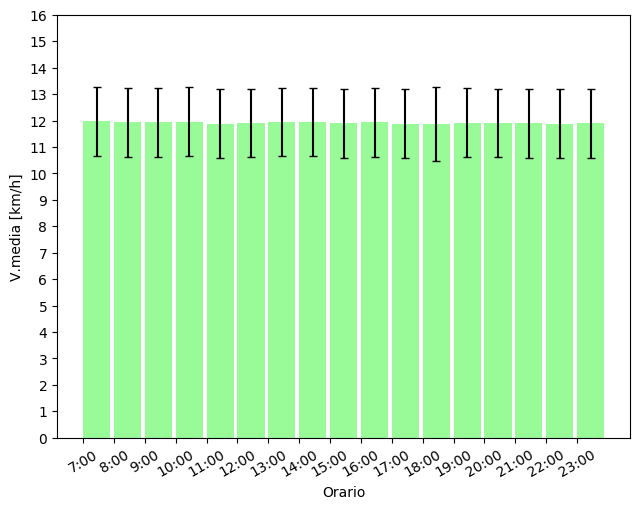
\includegraphics[scale=0.6]{vmedia_oraria_bici}
	\caption{Velocità media in bici [km/h] di ora in ora. I baffi neri rappresentano la deviazione standard campionaria $\sigma$ rispettiva di ogni barra}
	\label{image:11}
\end{figure}

\begin{figure}[H]
	\centering
	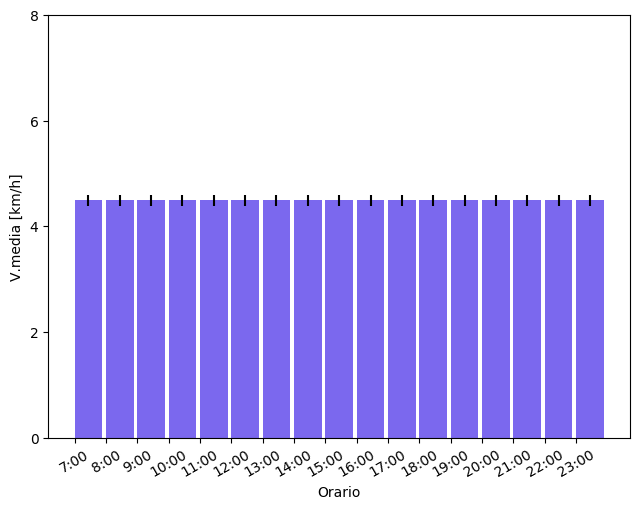
\includegraphics[scale=0.6]{vmedia_oraria_piedi}
	\caption{Velocità media a piedi [km/h] di ora in ora. I baffi neri rappresentano la deviazione standard campionaria $\sigma$ rispettiva di ogni barra}
	\label{image:18}
\end{figure}

\begin{figure}
\centering
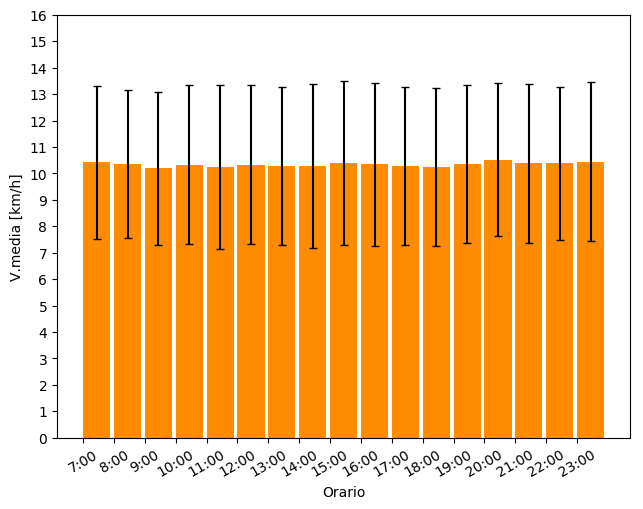
\includegraphics[scale=0.7]{vmedia_oraria_atm}
\caption{Velocità media coi mezzi pubblici [km/h] di ora in ora. I baffi neri rappresentano la deviazione standard campionaria $\sigma$ rispettiva di ogni barra}
\label{image:17}
\end{figure}

\begin{figure}
\centering
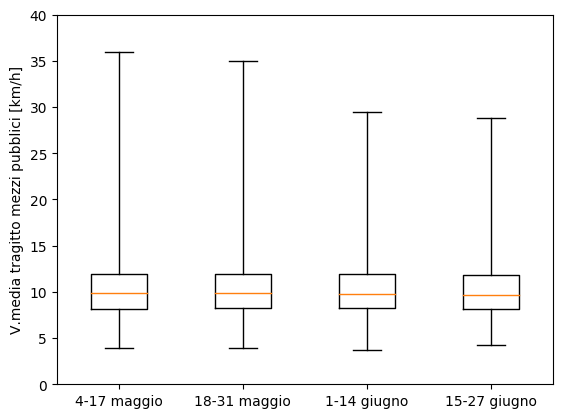
\includegraphics[scale=0.7]{vmedia_atm_weeks}
\caption{Distribuzione della velocità media coi mezzi pubblici [km/h] calcolata a gruppi di 2 settimane dalla fine del lockdown}
\label{image:29}
\end{figure}


\section{Confronto tra mezzi}

In questo paragrafo sono stati raccolti i risultati più interessanti emersi dal confronto tra tutti i mezzi di trasporto a disposizione per spostarsi nel Comune di Milano. Il confronto più atteso che ha fatto da guida verso questo studio è stato quello di verificare se, per un uso interno al Comune di Milano a solo scopo di spostamento e senza vincoli particolari come trasporto merci o passeggeri, l'automobile privata, insieme ai suoi svantaggi, potesse essere surclassata da un mezzo più economico e pulito come i mezzi pubblici in una città dove il traffico influisce in buona parte sui tempi di percorrenza, come mostrato nella Figura \ref{image:22}.

\subsection{Vittoria dell'automobile}

Nonostante la grande influenza del traffico sui tempi di percorrenza, i tragitti in auto sono risultati sempre i più veloci di ogni sua controparte, a qualsiasi ora del giorno e su ogni distanza, con una vittoria sopra il 99\% delle volte.

\subsection{Parziale sconfitta del car sharing}

\subsubsection{Mezzi pubblici ATM vs. Enjoy}

I risultati del confronto tra i mezzi pubblici ATM e il servizio di car sharing Enjoy illustrati nella Tabella \ref{table:5} mostrano una percentuale di vittorie di circa il 9\%, dove per vittoria si intende che il tempo impiegato a percorrere una tratta coi mezzi pubblici è stato minore o uguale al tempo impiegato utilizzando il car sharing. Nel grafico della Figura \ref{image:13} viene visualizzata la distribuzione di queste vittorie di ora in ora. Si può notare come vicino alle ore di picco del traffico individuate nell'analisi delle performance dell'auto, ovvero le ore 8:00-10:00 e 17:00-20:00, si concentri la percentuale maggiore di sconfitte da parte del car sharing. Per esempio, su tutte le tratte richieste nelle ore 8:00, nell'11\% delle volte i mezzi pubblici hanno pareggiato o superato la performance del car sharing. Al contrario, al di fuori degli orari di picco del traffico, la percentuale di vittorie è vicina allo 0. Dalla Tabella \ref{table:5} si evince anche che dell'8.7\% di queste vittorie, circa metà di esse sono tratte brevi dai 2 ai 5 km.

\begin{table}
	\centering
	\begin{tabular}{ | r r r | }
		\hline
		& \textbf{Abs. freq.} & \textbf{\% win} \\
		\textbf{(2, 5] km} & 2072 & 4.2 \\
		\textbf{(5, 7] km} & 1512 & 3.1 \\
		\textbf{(7, 10] km} & 670 & 1.4 \\
		\hline
		\textbf{totale} & 4294 & 8.7 \\
		\hline
	\end{tabular}
	\caption{Vittoria dei mezzi pubblici su car sharing per lunghezza tratta}
	\label{table:5}
\end{table}

\begin{figure}
	\centering
	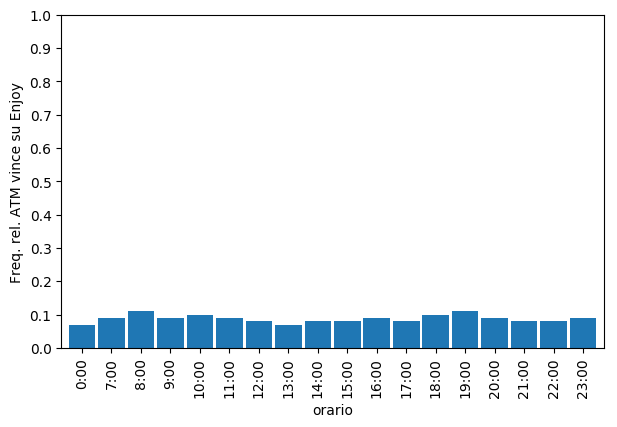
\includegraphics[scale=0.7]{confronto_atm_enjoy}
	\caption{Frequenza relativa vittorie ATM su Enjoy di ora in ora}
	\label{image:13}
\end{figure}

\subsubsection{Bicicletta vs. Enjoy}

Risultato ancora più interessante è quello del confronto tra bicicletta di proprietà e car sharing. La tabella \ref{table:6} mostra una percentuale delle vittorie del 36\% sul totale, poco più di un terzo del totale delle tratte. La maggior parte di queste vittorie è concentrata nelle tratte brevi dai 2 ai 5 km. Anche in questo confronto è emerso che negli orari di picco si accentua la percentuale di vittorie che arriva a toccare quasi il 45\% del totale nelle ore 8:00 e 18:00 come riportato dal grafico della Figura \ref{image:14}. Al contrario dei mezzi pubblici, questa percentuale resta alta anche al di fuori degli orari di punta, restando sempre intorno al 30\%.

\begin{table}[H]
	\centering
	\begin{tabular}{ | r r r | }
		\hline
		& \textbf{Abs. freq.} & \textbf{\% win} \\
		\textbf{(2, 5] km} & 15215 & 30.7 \\
		\textbf{(5, 7] km} & 2423 & 4.9 \\
		\textbf{(7, 10] km} & 278 & 0.6 \\
		\hline
		\textbf{totale} & 17917 & 36.2 \\
		\hline
	\end{tabular}
	\caption{Vittoria della bicicletta su car sharing per lunghezza tratta}
	\label{table:6}
\end{table}

\begin{figure}[H]
	\centering
	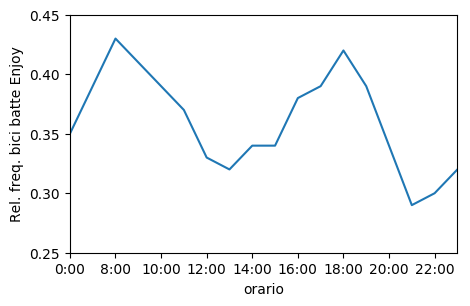
\includegraphics[scale=0.7]{confronto_bike_enjoy}
	\caption{Frequenza relativa vittorie bicicletta su Enjoy di ora in ora}
	\label{image:14}
\end{figure}

\pagebreak

\section{Confronto pre e post lockdown}

Nonostante le prime versioni del programma di raccolta dati abbiano portato a diversi errori nelle stime, quelle relative al percorso in automobile e car sharing sono sempre state corrette. Si è deciso quindi di analizzare l'unica settimana a disposizione prima del lockdown, dal lunedì 2 a domenica 8 marzo 2020, con una delle settimane più trafficate dopo il lockdown, che dalle analisi riportate dalle Figure \ref{image:5} e \ref{image:16} sono risultate corrispondenti al periodo dal 15 al 27 giugno 2020.

\subsection{Automobile}

Nel grafico della Figura \ref{image:22} si può notare una lieve differenza di km/h di media tra una settimana pre e post lockdown dal lunedì al venerdì. Questa differenza risulta più evidente negli orari di picco del traffico vicino alle 8:00 e alle 18:00, con una differenza di 2 km/h di media. Risulta evidente inoltre la differenza di velocità media nel pre lockdown tra le ore 8:00, dove si tocca il minimo di 17.5 km/h, e le ore 23:00, dove si trova il massimo di 24.5 km/h, una differenza di velocità del 28\%.

\subsection{Enjoy}

I tempi di percorrenza in car sharing Enjoy sono risultati molto simili, come mostrato dal grafico della Figura \ref{image:24}. La maggior differenza è presente anche questa volta vicino le ore di picco delle 8:00 e delle 18:00, sebbene la differenza sia minima, di media 1 km/h.

\begin{figure}[H]
	\centering
	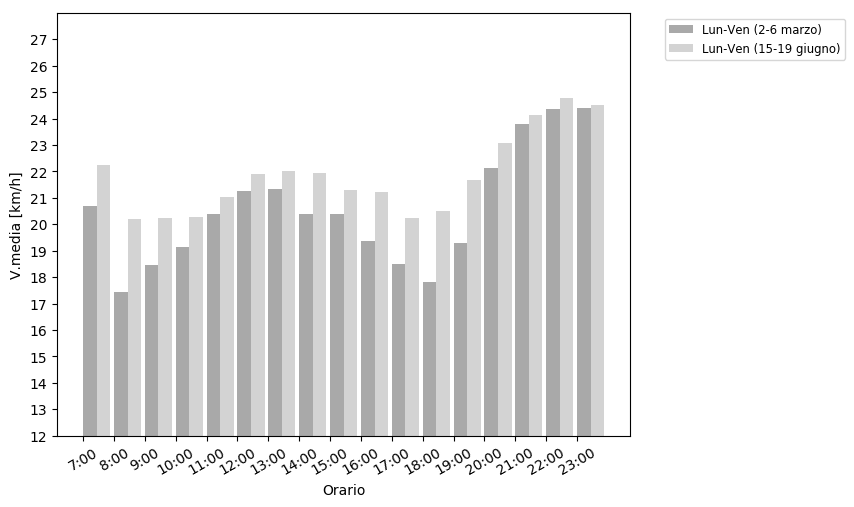
\includegraphics[scale=0.8]{vmedia_oraria_auto_prepostlock_week}
	\caption{Velocità media in auto [km/h] di ora in ora pre e post lockdown. I valori sull'asse delle ordinate variano tra 12 e 27}
	\label{image:22}
\end{figure}

\begin{figure}[H]
	\centering
	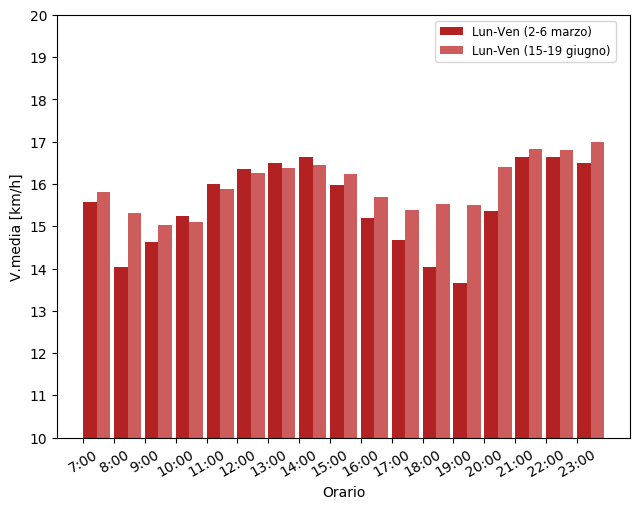
\includegraphics[scale=0.8]{vmedia_oraria_enjoy_prepostlock_week}
	\caption{Velocità media in Enjoy [km/h] di ora in ora pre e post lockdown. I valori sull'asse delle ordinate variano tra 10 e 20}
	\label{image:24}
\end{figure}












